\chapter{Design}
	
	\label{sec:design}
	
	The 3D Printing system can be divided up into three main parts as shown in
	figure \ref{fig:systemDiagramTop}. These major components and their
	requirements and design are described in the following sections.
	
	\begin{figure}
		\includegraphics[width=1\textwidth]{diagrams/systemDiagramTop.pdf}
		\caption{High-level diagram of overall system architecture.}
		\label{fig:systemDiagramTop}
	\end{figure}
	
	This project is principally focused on the development of the firmware and
	electronics used by the printer. In particular, the process of generating 3D
	models and G-code as well as mechanical operation is out of the scope of the
	project. The printer hardware and off-the-shelf, open source tools provided by
	the Makerbot project will be used for these purposes.
	
	\section{Firmware}
		
		The microcontroller firmware will consist of three main components running
		on top of the FreeRTOS operating system. The first will be the \uIP{}
		network stack for communication with the computer software. The second, is a
		G-code processing pipeline which will translate G-code into an appropriate
		sequence of commands to drive the electronics. The third component is a
		driver interface for the various Mbed peripherals.
		
		In this section, each of these components is examined followed by a brief
		discussion of the safety requirements of the system.
		
		\subsection{Network Interface}
			
			The firmware will provide an interface for streaming G-code to the printer
			and an interface for querying the printer's status. This will be done via
			a network interface primarily to increase the bandwidth of the connection
			with the computer.
			
			The G-code interface should be a simple open port which accepts G-code
			streams and feeds them into the pipeline without the need for specialised
			software on the sending computer. It will need to support flow control as
			the rate at which the printer is able to accept G-code instructions will
			vary depending on what instructions are being executed. For example, while
			waiting for heaters to warm up, no instructions are executed but during
			complex movements, many instructions are executed in rapid secession.  The
			interface must also be reliable because a missed, corrupted or
			out-of-order G-code instruction would cause potentially dangerous results.
			TCP offers both reliable communication and flow control mechanisms and is
			implemented in \uIP{} making it an appropriate choice for this
			task\footnote{Some G-code implementations have error checking and
			retransmission mechanisms built in but these are poorly specified and
			designed for use with serial connections.}.
			
			The status querying interface should be kept minimal and human readable. A
			\verb|telnet| compatible interface should be created.
		
		\subsection{G-code Processing Pipeline}
			
			The main task of the firmware is to process incoming G-code from the
			network and to control the printer appropriately without stalling. A
			pipeline architecture (figure \ref{fig:firmwarePipeline}) was selected
			where G-code from the network is buffered before being interpreted and
			converted into low-level commands. The low-level commands are placed in
			another buffer and then executed in sequence to drive the printer.
			
			\begin{figure}
				\includegraphics[width=1\textwidth]{diagrams/firmwarePipeline.pdf}
				\caption{G-code processing pipeline}
				\label{fig:firmwarePipeline}
			\end{figure}
			
			In order to reduce stalls due to data processing between commands, space
			is exchanged for computation time by keeping all command arguments in
			formats directly used by the printer in the low-level commands. For
			example, distances should be represented as an integral number of steps
			and not floating point millimetre values.
			
			At the start of the pipeline, the effect of network latency should be
			minimised by allocating a large G-code buffer giving the network longer to
			respond to changes in the rate of command execution before the buffer
			drains.
			
			Finally, by assigning a high priority to the printer controller the delay
			between a command completing and another starting is minimised.  This
			minimises the error introduced during very short bursts of extremely
			detailed movements.
		
		\subsection{G-code Interpreter}
			
			Though existing G-code interpreters are available they are generally
			tightly integrated with the control logic they were designed with and not
			easily used standalone. G-code implementations also vary widely with 3D
			printers but generally only a require a very small subset of the language
			features. As a result, a small G-code interpreter will be implemented for
			the required subset of G-code.
		
		\subsection{Drivers}
			
			In order to interface with the electronics and facilitate accurate timing,
			various peripherals on the Mbed will be used requiring supporting driver
			code. In particular, the following features will be needed:
			
			\begin{description}
				\item[General-Purpose Input/Output (GPIO)]
					Allows digital, TTL (Transistor-Transfer-Level), signals to be
					produced and read from the pins on the microcontroller. For example,
					stepper control and end-stop signals.
				
				\item[Analog Input]
					Read analog signals from the electronics, for example, readings from
					temperature sensors.
				
				\item[Timer]
					Used to produce interrupts at precisely timed intervals to allow
					stepper control signals to be generated.
				
				\item[Watch-dog Timer]
					To ensure fail-safe behaviour, a watch-dog timer can be used to reset
					and power down the system in the event of software malfunction.
			\end{description}
	
		\subsection{Safety}
			
			The system must behave safely in the event of a software failure and
			should be interruptible by a user at any time. The system must also start
			up in a safe state so that unintentionally powering on the machine cannot
			result in dangerous behaviour. Readings from the system must also be
			sufficiently accurate that they do not mislead the user about the system's
			safety.
	
	\section{Electronics \& Hardware}
		
		New electronics are required to replace the motherboard, relay and extruder
		boards. As well as this, electronics and hardware must be added for the
		proposed end-stop sensors. The requirements for these parts are described
		below.
		
		\subsection{Stepper Control}
			
			The printer's three primary axes are controlled by stepper motors which
			require complex circuitry to drive. Off-the-shelf RepRap stepper motor
			drivers (figure \ref{fig:stepperControllerBoard}) will be used as in the
			existing electronics \cite{stepperMotorDriver23}. The boards connect to
			the stepper motor and power supply and provide a TTL control interface.
			They also provide a connection for two end-stop sensors to be attached
			(the output from which they passively forward back through the TTL
			interface).
			
			\begin{figure}
				\includegraphics[width=1\textwidth]{diagrams/stepperControllerBoard.pdf}
				\caption{Stepper controller board with connections labelled. (Photo \cite{stepperControllerBoardPhoto})}
				\label{fig:stepperControllerBoard}
			\end{figure}
			
			The enable, direction and step signals from each stepper board must be
			driven by the microcontroller's GPIO pins.
		
		\subsection{Heater \& DC Motor Control}
			
			The heaters and motors both require large amounts of current at 12 volts
			to run. This far exceeds the output capabilities of the GPIO pins on the
			Mbed so a circuit will be needed to switch the power for these devices.
			
			Previously, mechanical relays were used to control the heaters but instead
			a solid-state solution should be sought to allow the posibility of varying
			heater power.
		
		\subsection{End-stops}
			
			By adding end-stop sensors on each axis, the axes can be accurately and
			consistently positioned at the start of a print job. Electronics
			compatible with the interface exposed by the stepper controller board will
			be required.
			
			Optical end-stops have been selected as the Makerbot has pre-drilled
			mounting holes at the end of each axis for mounting them.  Optical
			end-stops are also non-contact and so do not disrupt the movement of the
			axes.
